\subsection{Comparison: GRASP vs BRKGA}

In this section we are going to compare the performance of both metaheuristic algorithms applied to the assignment problem.\\
In order to do that, we are first going to choose the best parameters for each algorithm using the large set of problem instances described previously to execute several times each algorithm. The procedure consists of execution the same subset of samples drawn from the large set of problem instances for different proposed values of each parameter tested. The executions can be performed in different computers since the time is not important, only the objective function. The only caveat, is that all parameter values have to solve the same set of instances, since we use the average of objective functions. Otherwise the results would not be coherent from one parameter value to another. We record the objetive function for each execution and compute its average for each parameter value. Then we plot its evolution. We choose the parameter that produces the minimum objective function average.\\
Finally, we will use the best parameter values for each algorithm, to  compare the performance of both algorithm solving the same problem instance.


\subsubsection{Tuning GRASP parameters}

For the parameters of the GRASP algorithm, we have tested the $\alpha$, the $maxIterations$ of the main loop and the $failedIterations$ for the final and more intensive local search.\\
The results of the tests are shown in figure~\ref{fig_grasp_params} on page~\pageref{fig_grasp_params}.

\begin{figure}[h!]
\begin{subfigure}[b]{.49\linewidth}
\centering
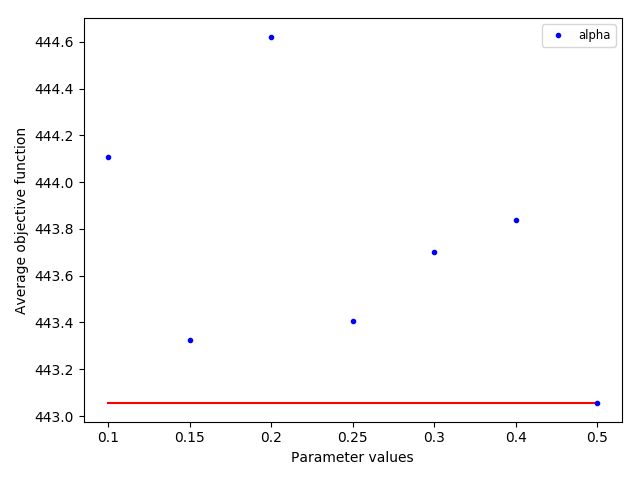
\includegraphics[width=0.8\linewidth]{./img/best-alpha.png}
\caption{ Parameter $\alpha$}\label{fig1a}
\end{subfigure}\hfill
\begin{subfigure}[b]{.49\linewidth}
\centering
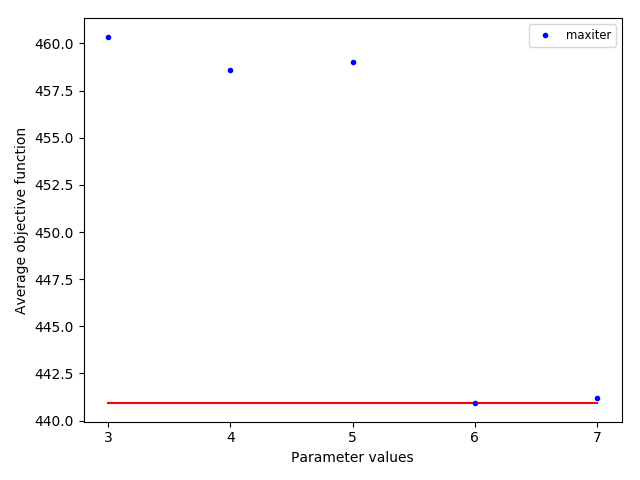
\includegraphics[width=0.8\linewidth]{./img/best-maxiter.png}
\caption{Parameter $maxIterations$ }\label{fig1b}
\end{subfigure}\vfill
\begin{subfigure}[b]{.49\linewidth}
\centering
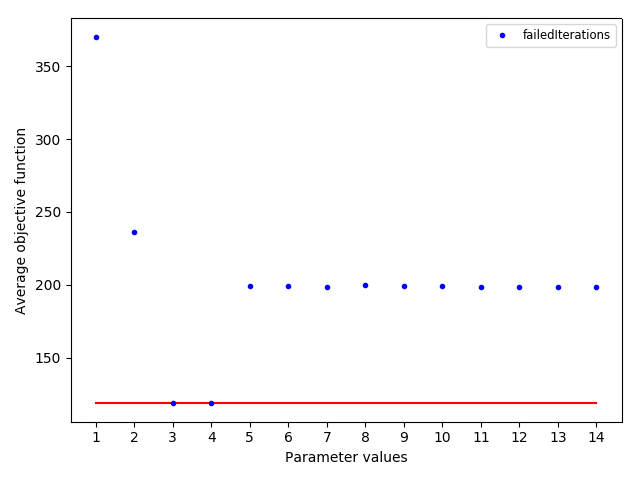
\includegraphics[width=0.8\linewidth]{./img/best-lsiteration.png}
\caption{Parameter $failedIterations$ }\label{fig1c}
\end{subfigure}%
\caption{Average objective function for different \subref{fig1a} $\alpha$, \subref{fig1b} $maxIterations$ and  \subref{fig1c} $failedIterations$ values.  }
\label{fig_grasp_params}
\end{figure}


\pagebreak

\subsubsection{Tuning BRKGA parameters}

For the parameters of the BRKGA algorithm, we have tested the number of generatons ($generations$), the number of individuals in the population ($population$), the inheritance probability ($inheritance$), the proportion of elite individuals in each generation ($eliteprop$) and the proportion of mutant individuals in each generation ($mutantprop$). The results of the tests are shown in figure~\ref{fig_brkga_params} on page~\pageref{fig_brkga_params} .\\

\begin{figure}[H]
\begin{subfigure}[b]{.49\linewidth}
\centering
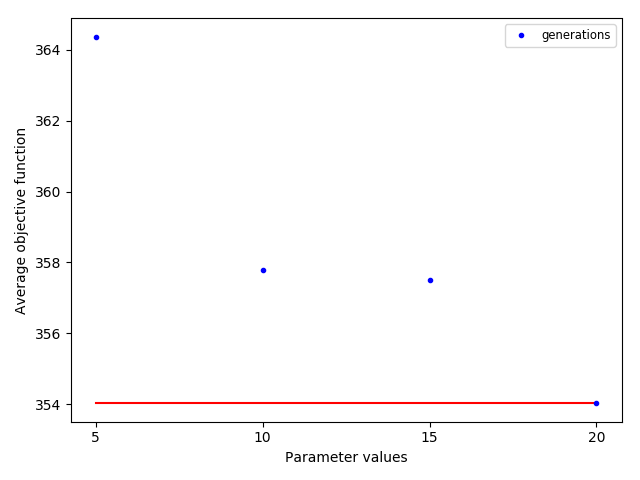
\includegraphics[width=0.8\linewidth]{./img/best-generation.png}
\caption{ Parameter $generations$}\label{fig2a}
\end{subfigure}\hfill
\begin{subfigure}[b]{.49\linewidth}
\centering
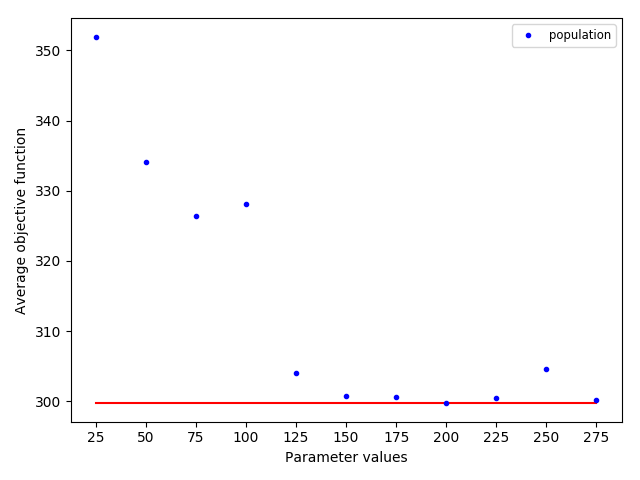
\includegraphics[width=0.8\linewidth]{./img/best-population.png}
\caption{Parameter $population$ }\label{fig2b}
\end{subfigure}\vfill
\begin{subfigure}[b]{.49\linewidth}
\centering
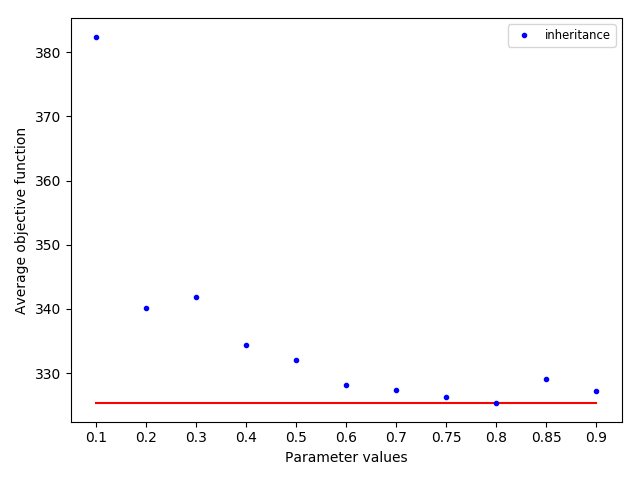
\includegraphics[width=0.8\linewidth]{./img/best-inheritance.png}
\caption{Parameter $inheritance$ }\label{fig2c}
\end{subfigure}%
\begin{subfigure}[b]{.49\linewidth}
\centering
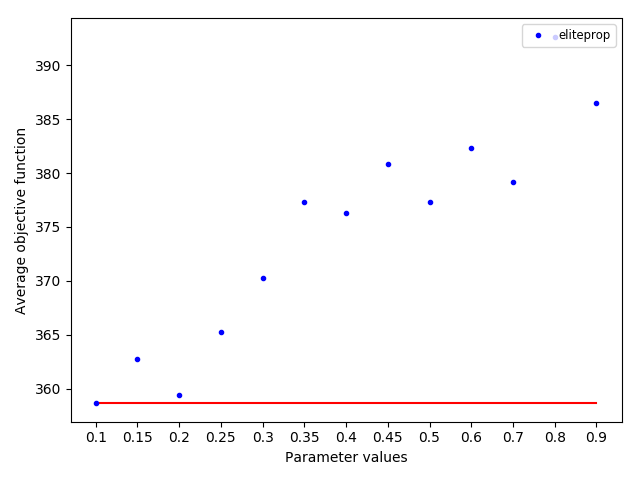
\includegraphics[width=0.8\linewidth]{./img/best-eliteprop.png}
\caption{Parameter $eliteprop$ }\label{fig2d}
\end{subfigure}\vfill
\begin{subfigure}[b]{.49\linewidth}
\centering
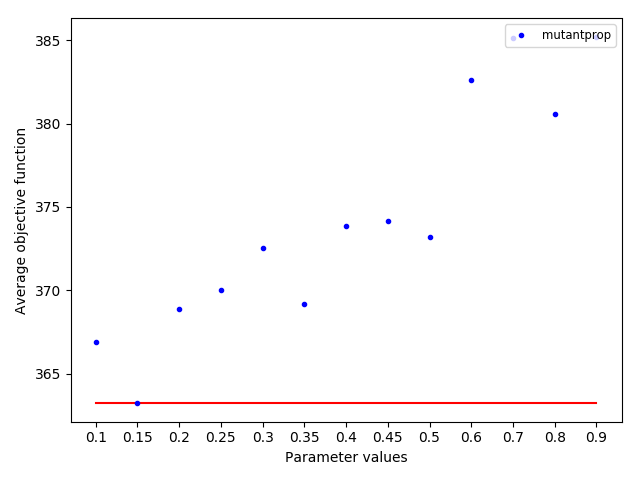
\includegraphics[width=0.8\linewidth]{./img/best-mutantprop.png}
\caption{Parameter $mutantprop$ }\label{fig2e}
\end{subfigure}%
\caption{Average objective function for different \subref{fig2a} $generations$, \subref{fig2b} $population$, \subref{fig2c} $inheritance$, \subref{fig2d} $eliteprop$ and \subref{fig2e} $mutantprop$ values.  }
\label{fig_brkga_params}
\end{figure}





\subsubsection{Comparative results of meta-heuristics performance}


Finally, we execute the same problem instance from the large set with both GRASP and BRKGA models. The selected problem instance is the following: \textbf{i-ng-60-4096-2560-24h-16mxP-4mxc-10mxH-1mnH-3Cnt-20180109\_08-04-50394.dat }


\begin{table}[h!]
  \centering
  \begin{tabular}{ m{5cm}  c   }

  	\textbf{GRASP}
	\begin{itemize}
		\item $\alpha$ = 0.25
		\item $maxIterations$ = 10
		\item $failedIterations$ = 4
	\end{itemize}

	\textbf{BRKGA}
	\begin{itemize}
		\item $generations$ = 12
		\item $population$ = 200
		\item $inheritance$ = 0.8 
		\item $eliteprop$ = 0.1
		\item $mutantprop$ = 0.15
	\end{itemize}


	&

  	\begin{minipage}{\textwidth}
	%\begin{figure}[h!]
	%\centering
	\begin{subfigure}[b]{.8\linewidth}
	%\centering
	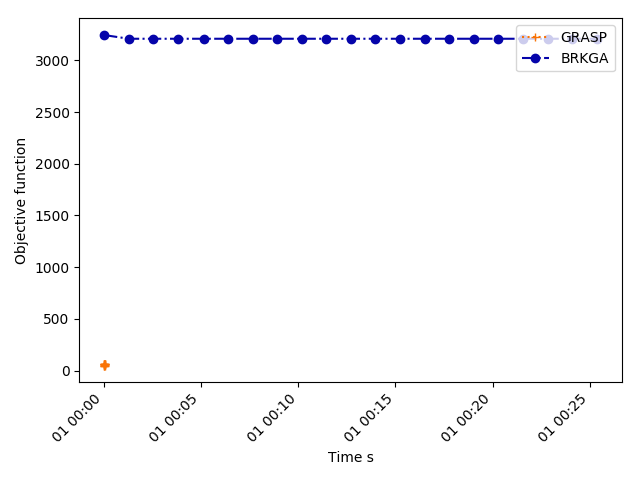
\includegraphics[width=0.8\linewidth]{./img/metah_comparison_objfunc.png}
	\end{subfigure}
	\end{minipage}


	 \\

  \end{tabular}
  \captionof{figure}{Objective function evolution by GRASP and BRKGA models using the best parameter setup.}\label{meta_comparison}
\end{table}


In the figure~\ref{meta_comparison} we observe that it takes the GRASP almost two more hours than BRKGA to finish. However, it finds a better local optimum (3190) than BRKGA(3209), except that both models find a local optimum around 3200 and the optimum is 2560.
The evolution of the objective function for the GRASP model shows a series of steps, that are combinations of the result of the Randomized Greedy constructive algorithm and then the Localsearch (which in most cases does not improve the solution). Then, around 2 hours from the beginning the objective function of the GRASP model starts to decrease. This is where the final intensive Localsearch algorithm is improving the solution (from the best pure Greedy or randomized Greedy constructive result). Because of the construction of the graph, the last Localsearch seems to improve from the last iteration of the Grasp ( Constructive plus Local search) but in fact it starts from the pure Greedy result at the very beginning. The final Localsearch does 36 iterations, starting at the best incumbent 3225 and decreasing slowly from 3222 to finally get an objective function value of 3190.

As we can observe in the chart, the BRKGA model finds the a local optimum in the fourth generation, but as it is setup to do twenty generations, it continues for 30 more minutes. This is caused by the fact that we have tested the parameters in isolation. We have not taken into account their interactions and strange results can appear like this early optimal finding of the BRKGA. An improvement that could be implemented is, as is done in the intensive localsearch, to introduce a limited number of non improving iterations upon which the algorithm stops. 
Looking at the diversity for each breed of individuals of the BRKGA model, we find that it starts with a rate of 30\% (61 different fitness values out of 200 individuals), increases to 41\% in the third generation then decreases to around 10\% and stays there. In the last generations it reaches 17\%, but the objective function stays the same as in the third generation where it finds the local optimum 3209.

In terms of intensification we can say that the final Localsearch of the GRASP algorithm does a good job, as well as the mating in the BRKGA's decoder. However the lightweight Localsearch during the GRASP iterations hasn't found improvements. 
In terms of diversification, this problem instance hasn't yield very impressive results. For example, the GRASP starts from 9 different constructive phases but they are close in terms of objective function. Moreover, the randomized constructive phases do not improve the pure Greedy approach so the space exploration capabilities of GRASP are not exploited as they could be. 

\pagebreak